\documentclass[11pt]{amsart}
\usepackage{geometry}                % See geometry.pdf to learn the layout options. There are lots.
\geometry{letterpaper}                   % ... or a4paper or a5paper or ... 
%\geometry{landscape}                % Activate for for rotated page geometry
%\usepackage[parfill]{parskip}    % Activate to begin paragraphs with an empty line rather than an indent
\usepackage{graphicx}
\usepackage{amssymb}
\usepackage{epstopdf}
\usepackage{hyperref}
\usepackage{float}
\DeclareGraphicsRule{.tif}{png}{.png}{`convert #1 `dirname #1`/`basename #1 .tif`.png}

\newcommand{\ra}{\ensuremath{\rightarrow}}

\title{Dissertation Proposal}
\author{Benjamin Berman}
%\date{}                                           % Activate to display a given date or no date

\begin{document}
\maketitle
%=======================================================================================
\section{Introduction}
%=======================================================================================

A long time ago my cello teacher pointed out that the way to play a difficult passage of music is not simply to grit one's teeth and keep practicing but to also figure out how to make playing those notes easy.  The major goal of the proposed dissertation is to reapply the same idea in the context of interactive theorem proving with the \textit{Coq} proof assistant\cite{Coq}\footnote{``Proof assistant'' and ``interactive theorem prover'' are synonymous}:  I intend to show ways to make the difficult task of using Coq easier by improving the user interface.  As well as solving serious usability problems for an important and powerful tool for creating machine-checked proofs, many of the techniques I am developing and testing are widely applicable to other forms of coding.

The research involved in this proposed dissertation, described more fully below, breaks down into two related main parts.  Part one is the development of ``CoqEdit'', a new theorem proving environment for Coq, based on the jEdit text editor.  CoqEdit will mimic the main features of the existing environments for Coq, but will have the important property of being easily extended using Java.  Part two is the development and testing of several such extensions.

There are several points that I hope will become clear as I describe the research for the proposed dissertation below.  First is that the research will make a significant positive contribution to society.  While Coq is a powerful tool, and is already being used for important work, its power has come at the cost of complexity, which makes the tool difficult to learn and use.  Finding and implementing better ways to deal with this complexity in the user interface of the tool can allow more users to perform a greater number, and a greater variety, of tasks.  At a more general level, the research contributes to a small but growing literature on user interfaces for proof assistants.  The work this literature represents can be viewed as an extension of work on proof assistants, which in turn can be viewed as an extension of work on symbolic logic:  symbolic logic aims to make working with statements easier, proof assistants aim to make working with symbolic logic easier, and user interfaces for proof assistants aim to make working with proof assistants easier.  These all are part of the (positive, I hope we can assume) academic effort to improve argumentative clarity and factual certainty.  
	
In addition, generalized somewhat differently, the research will contribute to our notions of how user interfaces can help people write code with a computer.  The complexities of the tool in fact help make it suitable for such research, since a) they are partly the result of the variety of features of the tool and tasks for which the tool may be used (each of which provides an opportunity for design) and b) the difficulties caused by the complexity may make the effects of good user interface design more apparent.  Furthermore, although Coq has properties that make it very appealing for developing programs (in particular, programs that are free of bugs), it also pushes at the boundaries of languages that programmers may consider practical for the time-constrained software development of the ``real world''.  However, if, as in the proposed research, we design user interfaces that address the specific problems associated with using a language, perhaps making the user interface as integral to using the language as its syntax, these boundaries may shift outward.  This means that not only are we improving the usability of languages in which people already are coding, we are also expanding the range of languages in which coding is actually possible.

The second point that I hope will become clear in this proposal is that this research will be an intellectual contribution, i.e. that the project requires some hard original thinking.  User interface development is sometimes ``just'' a matter of selecting some buttons and other widgets, laying them out in a window, and connecting them to code from the back end.  While this sort of work can actually be somewhat challenging to do right (just one of the hurdles is that testing is difficult to automate), the project goes well beyond this by identifying specific problems, inventing novel solutions, and testing these solutions in studies with human subjects.

The third and final point is that this work is actually doable.  Some of it has already been accomplished and the results will be described below.  The remaining work I also describe below, in enough detail, I hope, to make it seem reasonably straightforward. 

In the remainder of this proposal I will first give a description of Coq, including its significance, a description of current user interfaces, some examples of theorem proving using the tool, and some usability problems that I find particularly striking.  I will continue with a description of a survey, and its results, on user interfaces for Coq that was sent to subscribers to the Coq-Club mailing list.    Then, in the heart of this proposal, I will describe jEdit, CoqEdit, three experimental extensions to CoqEdit, and several associated user studies.  I will conclude with an overview of related work and a timeline for completing the remaining work.

%%=======================================================================================
\section{Coq and the Need for Improved User Interfaces}
%%=======================================================================================

%%================================
\subsection{Basic Theorem Proving in Coq}
\label{examplesection}
%%================================

Basic theorem proving in Coq can be thought of as the process of creating a ``proof tree'' of inferences.  The user first enters the lemma (or theorem) he or she wishes to prove.  The system responds by printing out the lemma again, generally in essentially the same form; this response is the root ``goal'' of the tree.  The user then enters a ``tactic''--a short command like ``apply more\_general\_lemma''--into the system, and the system will respond by producing either an error message (to indicate that the tactic may not be applied to the goal) or by replacing the goal with zero or more new child goals, one of which will be ``in focus'' as the ``current'' goal.  Proving all of these new child goals will prove the parent goal (if zero new child goals were produced, the goal is proved immediately).  Proving the current goal may be done using the same technique used with its parent, i.e. entering a tactic to replace the goal with a (possibly empty) set of child goals to prove, and which goal is the current goal changes automatically as goals are introduced and eliminated.  The original lemma is proved if tactics have successfully been used to create a finite tree of descendants--i.e. when there are no more goals to prove.

One example useful in making this more clear can be found in Huet, Kahn, and Paulin-Mohring's Coq tutorial \cite{huet1997coq}. Assume, for now, that we are just using Coq's read-eval-print loop, ``\texttt{coqtop}''.  Consider the lemma
\begin{equation}\label{exampleLemma}(A \ra B \ra C) \ra (A \ra B) \ra A \ra C\end{equation}
where of course $A$, $B$, and $C$ are propositional variables and ``\ra'' means ``implies'' and is right-associative\footnote{So this lemma is equivalent to $(A \ra (B \ra C)) \ra ((A \ra B) \ra (A \ra C))$} (I discuss later how improved user interfaces may assist users, particularly novice users, in dealing with operator associativities and precedences).  Assuming, also, that we have opened up a new ``section'' where we have told Coq that $A$, $B$, and $C$ are propositional variables, when we enter this lemma at the prompt, Coq responds by printing out
\begin{quote}
\texttt{ \\
%1 subgoals \\
A : Prop \\
B : Prop \\
C : Prop \\
\_\_\_\_\_\_\_\_\_\_\_\_\_\_\_\_\_\_\_\_\_\_\_\_\_\_\_\_\_\_\_\_\_\_\_\_\_\_ \\%(1/1) \\
(A -> B -> C) -> (A -> B) -> A -> C \\}

\end{quote}


% Consider a lemma, call it \texttt{SimpleLemma} that states
%\begin{quote}
%\texttt{(A -> B -> C) -> (A -> B) -> A -> C}
%\end{quote}
%where \texttt{A}, \texttt{B}, and \texttt{C} are propositions (abbreviated in Coq as ``\texttt{Prop}''), and \texttt{->} is interpreted as ``implies'' and is right %associative (so the lemma may equivalently be written 
%\begin{quote}
%\texttt{(A -> (B -> C)) -> ((A -> B) -> (A -> C))}
%\end{quote}
%I discuss later how improved user interfaces may assist users, particularly novice users, in dealing with operator associativities and precedences).  Coq users generally think of this lemma as the sequent
For the purposes of this example, I will write such ``sequents'' using the standard turnstile ($\vdash$) notation.  The response then becomes: 
\begin{equation}\label{initialGoal}A : Prop, B : Prop, C : Prop \vdash (A \ra B \ra C) \ra (A \ra B) \ra A \ra C\end{equation}
%\[A : Prop, B : Prop, C : Prop \vdash (A \ra B \ra C) \ra (A \ra B) \ra A \ra C\]

In general, the statements to the left of the $\vdash$, separated by commas, give the ``context'' in which the provability of the statement to the right of the turnstile is to be considered.\footnote{Another list of statements, Coq's ``environment,'' is implicitly to the left of the turnstile.  The distinction between environment and context is that statements in the context are considered true only locally, i.e. only for either the current section of lemmas being proved or for the particular goal being proved.  Generally, the environment is large, and contains many irrelevant statements, so displaying it is considered impractical.}  Another way to think about the sequent is that the statements to the left of the turnstile entail the statement to the right (or, at least, that is what we would like to prove).  In this example sequent's context, the colon indicates type, so for instance ``$A : Prop$'' just means ``$A$ is a variable of type $Prop$'' or, equivalently, ``$A$ is a proposition.''

Note that this is an extremely simple example; one could actually use Coq's \texttt{auto} tactic to prove it automatically.  Theorems and lemmas in Coq typically involve many types and operators besides propositions and implications.  Other standard introductory examples involve natural numbers and lists, along with their associated operators and the other usual operators for propositions (e.g. negation).  In fact, Coq's \textit{Gallina} language allows users to declare or define variables, functions, types, constructors for types, axioms, etc., allowing users to model and reason about, for instance, the possible effects of statements in a programming language, or more general mathematics like points and lines in geometry.

The sequence of tactics, ``\texttt{intro H}'', ``\texttt{intros H' HA}'', ``\texttt{apply H}'', ``\texttt{exact HA}'', ``\texttt{apply H'}'', and finally ``\texttt{exact HA}'' can be used to prove the sequent above (\texttt{H}, \texttt{H'}, and \texttt{HA} are arguments given to \texttt{intro}, \texttt{intros}, \texttt{apply}, and \texttt{exact}).  The first tactic, ``\texttt{intro H}'', operates on \eqref{initialGoal}, moving the left side of the outermost implication (to the right of the turnstile) into the context (i.e. the left side of the turnstile).  The new subgoal, replacing \eqref{initialGoal}, is
\begin{equation}\label{introHResult}A : Prop, B : Prop, C : Prop, H : A \ra B \ra C \vdash (A \ra B) \ra A \ra C\end{equation}
%\[A : Prop, B : Prop, C : Prop, H : A \ra B \ra C \vdash (A \ra B) \ra A \ra C\]
The colon in the statement ``$H : A \ra B \ra C$'' is generally interpreted differently, by the user, than the colons in ``$A : Prop, B : Prop, C : Prop$''.  Instead of stating that ``$H$ \textit{is of type} $A \ra B \ra C$'', the user should likely interpret the statement as ``$H$ \textit{is proof of} $A \ra B \ra C$''.  However, for theoretical reasons, namely the Curry-Howard correspondence between proofs and the formulas they prove, on the one hand, and terms\footnote{``Terms,'' such as the ``$A$'' in ``$A : Prop$'', are roughly the same as terminating programs or subcomponents thereof; they may be evaluated to some final value.  Note also that the types of terms are terms themselves and have their own types (not all terms are types, however).  A type of the form $\it{\Phi} \ra \it{\Theta}$, where both $\it{\Phi}$ and $\it{\Theta}$ are types that may or may not also contain \ra symbols, is the type of a function from terms of type $\it{\Phi}$ to terms of type $\it{\Theta}$.  For instance, a term of type $nat \ra nat$ would be a function from natural numbers to natural numbers.} and types they inhabit, on the other, Coq is allowed to ignore this distinction and interpret the colon uniformly.  If fact, in proving a theorem, a Coq user actually constructs a program with a type corresponding to the theorem.  This apparent overloading of the colon operator may be a source of confusion for novice users and while there are no plans in this proposal for directly mitigating the confusion, extensions to the proposed user interface might do so by marking which colons should be interpreted in which ways.  Furthermore, by clarifying other aspects of the system, we hope to free up more of novice users' time and energy for understanding this and other important aspects of theorem proving with Coq that we may not be able to address. 

Tactics allow users to reason ``backwards''--if the user proves the new sequents(s), then the user has proved the old sequent.  In other words, the user is trying to figure out what could explain the current goal, instead of trying to figure out what the current goal entails.\footnote{Another possible point of confusion for novice users:  when the differences between the old and new sequents are in the contexts, rather than the succedents (i.e. on the left of the turnstiles rather than on the right) we may say we are doing forward reasoning, even though we are still adding new goals further away from our root goal.  This may make most sense when one views a sequent as a partially completed Fitch-style proof--this forward reasoning is at the level of statements within sequents, rather than at the level of sequents.}  Above, the (successful) use of the ``\texttt{intro}'' tactic allows the user to state that {\bf if} in a context where $A$, $B$, and $C$ are propositions \textit{and} $A \ra B \ra C$ it is the case that $(A \ra B) \ra A \ra C$, {\bf then} in a context containing only that $A$, $B$, and $C$ are propositions it is the case that $(A \ra B \ra C) \ra (A \ra B) \ra A \ra C$.  The fact that the tactic produced no error allows the user to be much more certain of the truth of this statement than he would if he just checked it by hand.\footnote{In general some uncertainty remains when using computer programs to check proofs. One danger is the possibility of mistranslating back and forth between the user's natural language and the computer program's language--this might happen, for instance, if a novice user were to assume an operator is left-associative when it is actually right-associative.  Another related danger, perhaps even more serious, is the possibility of stating the wrong theorem, or set of theorems.  For instance, a user might prove that some function, $f$, never returns zero, but that user might then forget to prove that some other function, $g$, also never returns zero.  An important role of theorem prover user interfaces is to mitigate these dangers by providing clear feedback and by making additional checks easier (e.g. quickly checking that $f(-1) = 1$, $f(0) = 1$, and $f(1) = 3$ might help the user realize that the property of $f$ that he actually wants to prove is that its return value is positive, not just nonzero).}

%proving that various functions defined in terms of $f$ and $g$ have the properties we expect them to have gives us additional confidence that $f$ and $g$ are acceptably defined).

%the possibility of misstating the theorem to be proved, for instance, is a serious danger

The tactic ``\texttt{intros H' HA}'' is equivalent to two intro tactics, ``\texttt{intro H'}'' followed by ``\texttt{intro HA}'', so it replaces \eqref{introHResult} with
\begin{equation}\label{introsResult}A : Prop, B : Prop, C : Prop, H : A \ra B \ra C, H' : A \ra B,  HA : A \vdash C\end{equation}
%\[A : Prop, B : Prop, C : Prop, H : A \ra B \ra C, H' : A \ra B,  HA : A \vdash C\]

Next, the tactic ``\texttt{apply H}'' replaces \eqref{introsResult} with \textit{two} new subgoals:
\begin{equation}\label{applyHresult1}A : Prop, B : Prop, C : Prop, H : A \ra B \ra C, H' : A \ra B,  HA : A \vdash A\end{equation}
%\[A : Prop, B : Prop, C : Prop, H : A \ra B \ra C, H' : A \ra B,  HA : A \vdash A\]
and
\begin{equation}\label{applyHresult2}A : Prop, B : Prop, C : Prop, H : A \ra B \ra C, H' : A \ra B,  HA : A \vdash B\end{equation}
%\[A : Prop, B : Prop, C : Prop, H : A \ra B \ra C, H' : A \ra B,  HA : A \vdash B\]
This successful use of ``\texttt{apply H}'' says that the proof $H$, that $A \ra (B \ra C)$, (parentheses added just for clarity) can be used to prove $C$, but, in order to do so, the user must prove both $A$ and $B$.  Note that, in contrast with use of the \texttt{intro} tactic, after using the \texttt{apply} tactic the contexts has not changed.  Also note that the first of these two becomes the current goal.

The next tactic, ``\texttt{exact HA},'' eliminates \eqref{applyHresult1}, not replacing it with any new goal (if there is already proof of \texttt{A}, in this case \texttt{HA} in the context, then there is nothing left to do;  ``\texttt{apply HA}'' would have the same effect), and focus moves automatically to \eqref{applyHresult2}.  The tactic ``\texttt{apply H'}'' replaces \eqref{applyHresult2} with a new goal, but this new goal is identical to \eqref{applyHresult1} (we can use $A \ra B$ to prove $B$ if we can prove $A$), and so ``\texttt{exact HA}'' can be used again to to eliminate it.  Since there are no more goals, the proof is complete.

%%================================
\subsection{Coq's Significance}
%%================================

The example above is intended to give some sense of what interactive theorem proving with Coq is all about, and the complexities that novice users face, but it barely scratches the surface of Coq's full power and complexity.  It also does little to suggest Coq's significance.    Most of the applications accounting for this importance can be divided into those relating (more directly) to computer science and those relating to mathematics.\footnote{See the categorization of user contributions on the Coq website:  http://coq.inria.fr/pylons/pylons/contribs/bycat/v8.4}

On the computer science side, Coq has an important place in research on ensuring that computer software and hardware is free of bugs.  Given the increasing use of computers in areas where bugs (including security vulnerabilities) can have serious negative consequences (aviation, banking, heath care, etc.), such research is becoming increasingly important.  Given, also, that exhaustive testing of the systems involved in these areas is generally infeasible, researchers have recognized the need to actually prove the correctness of these systems (i.e. that the systems conform to their specifications). While fully-automatic SAT solvers (for propositional satisfiability) and SMT (satisfiability modulo theory) solvers are being used to implement advanced static analysis techniques with promising results (e.g. \cite{gulwani2008program,dillig2011small}) and can determine the satisfiability of large numbers of large formulas, keeping humans involved in the theorem proving process allows the search for a proof to be tailored to the particular theorem at hand, and therefore allows a wider range, in a sense, of theorems to be proved.  Furthermore, contrary to what might have been suggested by the step-by-step detail of the example above, many subproblems can be solved automatically by Coq and other interactive theorem provers, and work is being done to send subproblems of interactive theorem provers to automatic tools \cite{bohme2010sledgehammer} in order to combine the best of both worlds.  Notable computer science-related achievements, some in industrial contexts, for Coq and other interactive theorem provers include verification of the seL4 microkernel \cite{klein2010sel4} in Isabelle\cite{Isabelle}, the CompCert verified compiler\cite{leroy2009formal} for Clight (a large subset of the C programming language) in Coq, Java Card EAL7 certification\cite{gemaltogemalto} using Coq, and, at higher levels of abstraction, verification of the type safety of a semantics for Standard ML \cite{lee2007towards} using Twelf\cite{Twelf} and use of the CertiCrypt framework \cite{CertiCrypt} built on top of of Coq to verify cryptographic protocols (e.g. \cite{barthe2010machine}).\footnote{An earlier version of this paragraph, from which come most of the included references, was written by Dr. Aaron Stump for an unpublished research proposal.  Many of the references from the next paragraph also come from this proposal.}

On the mathematics side, Coq is being used to formalize and check proofs of a variety of mathematical sub-disciplines, as demonstrated by user contributions listed on the Coq website.  Perhaps Coq's most notable success story is its use in proving the Four Color Theorem \cite{gonthier2005computer}.  Other interactive theorem provers are also having success in general mathematics.  For instance, Matita \cite{Matita}, which is closely related to Coq, was used in a proof of Lebesgue's dominated convergence theorem \cite{coen2008constructive}.  There are in fact efforts to create libraries of formalized, machine-checked mathematics, the largest of which is the Mizar Mathematical Library \cite{geuvers2009proof}.  ITPs are also a potential competitor for computer algebra systems (e.g. Mathematica) with the major advantage that they allow transparency in the reasoning process, a significant factor limiting computer algebra use in mathematics research according to \cite{bunt2009friend}.

The potential for transparency also helps make interactive theorem provers, like Coq, a potentially useful tool in mathematics, logic, and computer science education.  Rather than simply giving students the answers to homework problems, interactive theorem provers might be used to to check students' work, find the precise location of errors and correct misconceptions early.  Interest in adapting theorem provers for educational purposes can be seen in many references listed later in this document; Benjamin Pierce et al.'s \textit{Software Foundations}\cite{pierce2010software}, a textbook, written mostly as comments in files containing Coq code and which includes exercises having solutions that may be checked by Coq, serves as an example of how the tool can be effectively used in education.  More general interest in educational systems that check student work can be seen in logic tutorial systems such as ``P-Logic Tutor'' \cite{lukins2002tutorial}, ``Logic Tutor'' \cite{lesta2002intelligent}, ``Fitch'' (software accompanying the textbook \textit{Language, Proof, and Logic} \cite{barwise2000language}), and ``ProofMood''\cite{ProofMood}.

The part of the case for Coq's significance that is presented above is more a case for interactive theorem provers in general than Coq in particular; after reading it one may wonder, why try to improve Coq usability instead of usability for some other proof assistant?  The answer is that it is already one of the most powerful and successful such tools.  Adam Chlipala, in the introduction to his book \textit{Certified Programming with Dependent Types} \cite{chlipala2011certified}, presents a list of major advantages over other proof assistants in use:  its use of a higher-order language with dependent types, the fact that it produces proofs that can be checked by a small program (i.e. it satisfies the ``de Bruijn criterion''), its proof automation language, and its support for ``proof by reflection.''
\footnote{Basically, this is proof by providing a procedure to get a proof.  Coq allows one to prove that these procedures produce correct proofs.}  As evidence of its resulting success, note that Coq was awarded the 2013 ACM SIGPLAN Programming Languages Software Award \cite{CoqSIGPLANAward}.

%%================================
\subsection{Current User Interfaces and Problems They Present to Novice Users}
\label{currentUIproblems}
%%================================

The example presented earlier can be used to illustrate some more of the common challenges for users.  For novice users, one of the biggest challenges is to discover exactly what Coq's tactics do when applied to various arguments and goals.   Only four tactics were used in the example, but many more are standard (the Coq Reference Manual\cite{Coq:manual} lists almost 200 in its tactics index), and Coq allows new tactics to be defined.  Other challenges, for both novice and expert users, will be discussed below, but the lack of support for users trying to understand tactic effects is, by itself, probably sufficient justification for the development of new user interfaces.

The two major user interfaces for Coq are currently \textit{Proof General}\cite{ProofGeneral,aspinall2000proof} and \textit{CoqIDE} (which is available from the Coq website\cite{Coq}, and is bundled with Coq).  Interacting with Coq using one is quite similar to interacting with Coq using the other, the main difference being that Proof General is actually an Emacs mode (and so has the advantages and disadvantages of the peculiarities of the Emacs text editor, e.g. numerous shortcuts and arguably a steep learning curve).

\begin{figure}[h]
  \center
  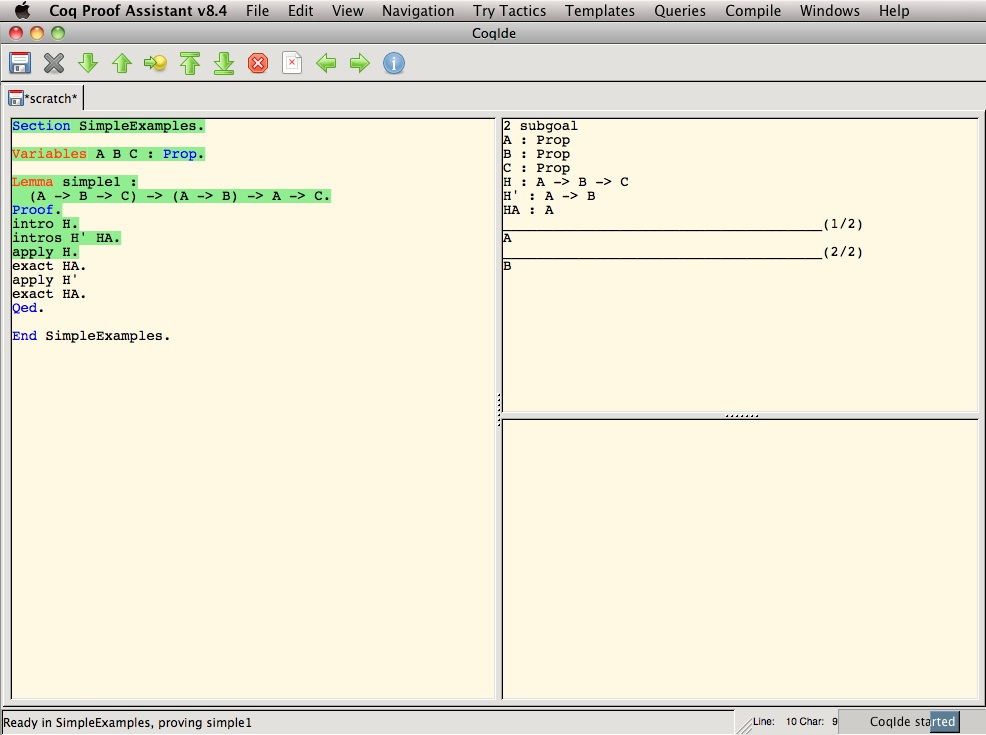
\includegraphics[width=\linewidth]{simple1_1.jpg}
  \caption{CoqIde, displaying the result of entering the tactic ``\texttt{apply H}'' in the top-right panel within the proof of \texttt{(A -> B -> C) -> (A -> B) -> A -> C}.}
  \label{fig:simple1_1}
\end{figure}

\begin{figure}[h]
  \center
  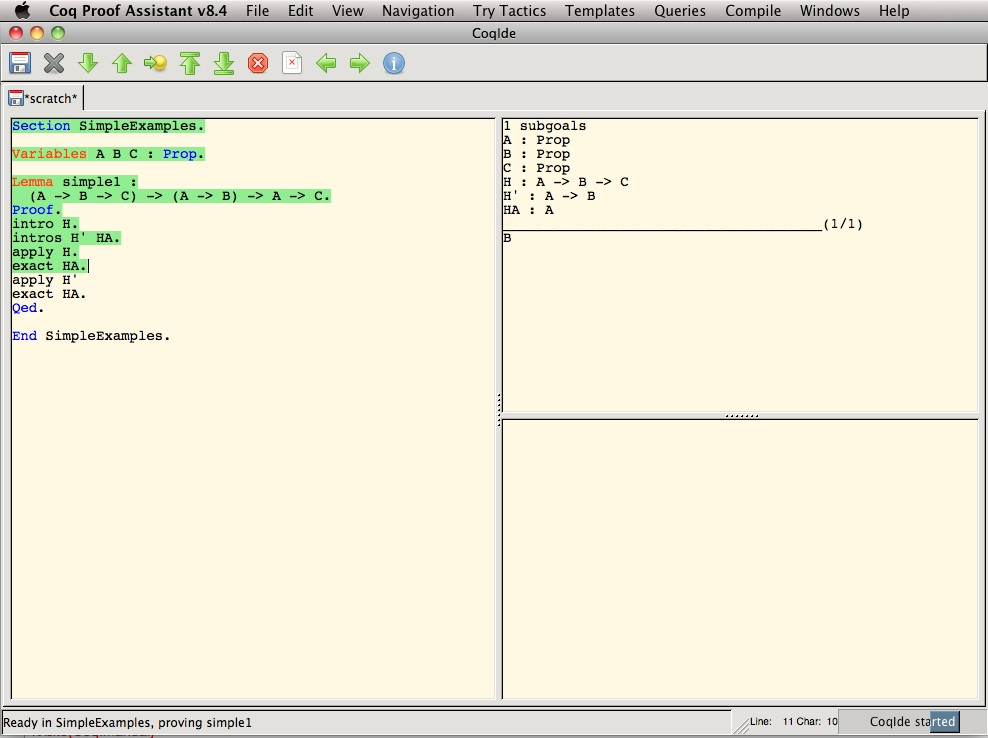
\includegraphics[width=\linewidth]{simple1_2.jpg}
  \caption{CoqIde after moving the end of the evaluated portion of the script forward by one sentence from the state shown in \autoref{fig:simple1_1}.}
  \label{fig:simple1_2}
\end{figure}


\autoref{fig:simple1_1} and \autoref{fig:simple1_2} show the CoqIde user interface as it appears while entering the proof from the the earlier example, that $(A \ra B \ra C) \ra (A \ra B) \ra A \ra C$,  into Coq.\footnote{Note that ``\texttt{simple1}'', in ``\texttt{Lemma simple1 : (A -> B -> C) -> (A -> B) -> A -> C.}'', is the identifier we are binding to the \textit{proof} of the lemma, and not to the lemma itself.  Without recognizing this, the fact that the keyword ``\texttt{Lemma}'' could have been replaced by the keyword ``\texttt{Definition}'' may be yet another source of confusion since it suggests that Coq thinks lemmas and definitions are basically the same thing!  As one might expect, we could also bind an identifier to the lemma itself.  If we were to bind the identifier ``\texttt{SimpleLemma}'' to this lemma, we would most likely use the \texttt{Definition} keyword in combination with ``\texttt{:=}'', and write \\``\texttt{Definition (SimpleLemma : Prop) := (A -> B -> C) -> (A -> B) -> A -> C.}''}  
The larger panel on the left shows a script that will, in general, contain definitions, theorems, and the sequences of tactics used to create proofs of these theorems.\footnote{Here the declaration of A, B, and C, and the definition of the proof of the lemma are within a section that has been named ``\texttt{SimpleExamples}.''  This sets the scope A, B, and C to just the section.  Outside of the section, reference to simple1 is allowed.  However, simple1 is changed to a proof that $\forall (A : Prop), (\forall (B : Prop), (\forall (C : Prop), ((A \ra B \ra C) \ra (A \ra B) \ra A \ra C)))$, generally written \texttt{forall A B C : Prop, (A -> B -> C) -> (A -> B) -> A -> C}.}
A portion of this script, starting at the beginning, may be highlighted in green to show that it has been successfully processed by Coq. Another portion of the script, following this green highlighting or starting at the beginning if there is no green highlighting, may be highlighted in blue to show where the ``sentences'' of the script are either being evaluated or have been queued for evaluation (sentences in the script are separated by periods followed by whitespace, as in English).  Whenever Coq is not already processing a sentence, and there are queued sentences, the first sentence in the queue is automatically dequeued and sent to Coq, i.e. if there is a first blue-highlighted sentence, Coq is trying to evaluate it.

If a sentence is successfully processed, its highlighting changes to green and the output resulting from the successful processing is printed in one of the two panels on the right side of the window.  Assuming the system is in ``proof mode'' (e.g. after processing the sentence ``\texttt{Lemma simple1}...'' in \autoref{fig:simple1_1} and \autoref{fig:simple1_2}, but before evaluating ``\texttt{Qed.}''), the top panel displays the current goal, including its context, followed by just the consequents of any remaining goals.  The bottom panel is used to display various messages, e.g. error message and acknowledgements of successful definitions. Otherwise, if processing of a sentence results in an error, all sentences queued for processing are removed from the queue, the blue highlighting representing that queue is removed, and the font of the offending part of the offending sentence is changed to bold, underlined red.  In general, processing a sentence is not guaranteed to produce a result of any kind (error or otherwise) in any specified amount of time (some sentences are semi-decision procedures), so CoqIde allows users to interrupt the processing of a sentence.  This also has the effect of removing all sentences from the processing queue and removing all blue highlighting. Frequently, however, processing is fast enough that the blue highlighting never even becomes actually visible.

Users can extend the highlighted region both forward, to evaluate unhighlighted sentences, and backwards, to undo the effects of evaluation.  Users can instruct the system to extend the highlighting forward by one sentence, to retract it back by one sentence (though in the latest version of Coq, this sometimes will actually move the highlighting back several sentences), to extend or retract it to the cursor, to remove all of it (i.e. retract it to the start of the script), and to extend it to the end of the script.  These instructions can be entered into the system using toolbar buttons, drop-down menu items, or keyboard shortcuts.

\autoref{fig:simple1_1} and \autoref{fig:simple1_2} illustrate some of these points.  In \autoref{fig:simple1_1}, in the top right, we see the the result of evaluating ``\texttt{apply H}''.  In \autoref{fig:simple1_2}, we see the highlighting extended and the result of ``\texttt{exact HA} in the top right--the elimination of the first of the two subgoals in \autoref{fig:simple1_1} and the change in focus to the second.

This interface is problematic for novices trying to learn the effects of tactics.  Unfortunately, because the particular example being discussed is so simple, the severity of the problem may not be immediately apparent.  In \autoref{fig:simple1_1}, the two goals resulting from using the tactic ``apply H'' (the statement at the end of the highlighted region) appear to be displayed in the top right panel.  In fact, as mentioned earlier, only the first goal is fully displayed--the context for the second is not.  (In this case, the contexts for both are identical, but this is not always what happens).  To see the context of the second goal, probably the easiest, or at least most natural, thing for the user to do is highlight forward through all the tactics used to prove the first goal (just one tactic here, but potentially many in general).  It is up to the user to determine how far to highlight (or un-highlight, if looking at an earlier sibling goal) by keeping track of the list of goals in the top-right panel.  

In addition to the problem of moving through the script to fully see siblings, note that no distinction is made between sibling and non-sibling goals in the list presented.  For instance, instead of using ``\texttt{exact HA}'' to transition to \autoref{fig:simple1_2}, the user could have used a tactic that produced two new goals.  The list of goals would then contain three goals, but only the first two would be siblings.  The user interface leaves it up to the user, however, to determine this by keeping track of the number of goals.\footnote{This sort of debugging gets even harder when one introduces proof automation features that allow combinations of basic tactic use attempts.}

Proof general does introduce a few features not present in CoqIde.  For instance, instead of making the highlighted region un-editable (``locking'' it), typing in the highlighted region retracts the highlighting back to the end of the sentence immediately before the cursor.  Unfortunately, these features are not really aimed at showing the effects of tactics.  A third user interface, \textit{Proof Web}\cite{ProofWeb} does make a serious attempt.  ProofWeb, for the most part, is a web-based version of CoqIde.  However, it has a major improvement, shown in the bottom right of \autoref{fig:proofweb}: a visualization of the partially completed proof tree.  

ProofWeb's display of the tree follows the convention where inferences are drawn with a horizontal line separating horizontally listed premises, above, from the conclusion below, and where each horizontal line is labeled with the name of the corresponding inference rule (or, in the case of Coq, by the corresponding tactic name) to the right of the line.  These inferences can be chained together so that the root of the proof tree is drawn at the bottom and the leaves are drawn at the top.  As an example, the portion of the proof tree constructed by ProofWeb that corresponds to ``\texttt{apply H}'' is shown in \autoref{fig:applyH} (the ellipses indicate that the child nodes are still unproved), and \autoref{fig:fulldisplaypartialtree} fully displays the partially completed tree.  The user is able to much more directly see the goal to which \texttt{apply H} is applied and the goals this application produces.

\begin{figure}[h]
  \center
  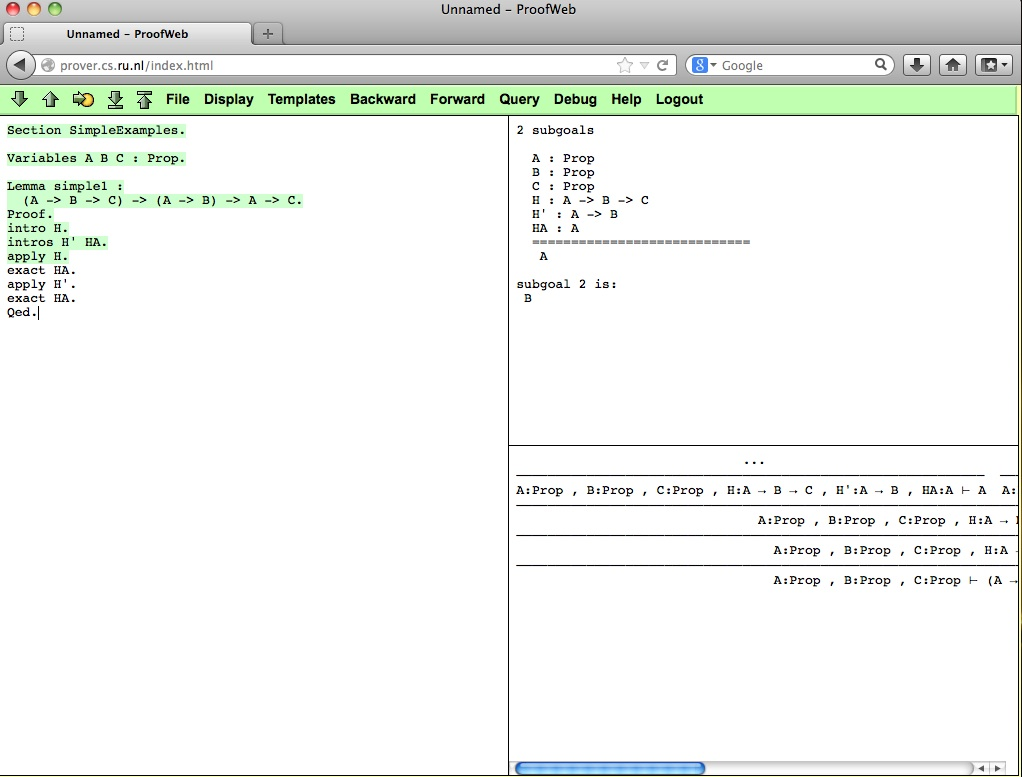
\includegraphics[width=\linewidth]{ProofWeb.jpg}
  \caption{ProofWeb, with a partial proof tree displayed in the bottom right.}
  \label{fig:proofweb}
\end{figure}



Unfortunately, as one can probably already tell, this sort of visualization does not scale particularly well.\footnote{Later in this document I provide what I hope is a clearly better alternative.} Contexts may may have dozens of items, many of which may be much longer than ``\texttt{H : A -> B -> C}, and the number of nodes in the proof tree may also be very large.  As a result, to see the effect of a tactic the user may have to pan around the window; this is especially likely if one is looking at a tactic used near the root of the tree, since the width of the tree at its leaves forces apart nodes near the root.  Even if the user does not need to pan (ProofWeb has a feature that allows the tree to be displayed in a separate window, which can sometimes make panning unneccessary), the distances at which nodes with sibling and parent-child relationships must sometimes be placed may make it difficult for the user to compare such sequents and to determine if a direct relationship in fact exists (e.g. determine if two sequents that printed next to one another are siblings or ``cousins'').  The latter task is possibly especially difficult using this visualization since it involves checking for gaps in co-linear line segments and the human brain tends to connect such lines.\footnote{This is the Gestalt law of ``good continuation; see, for instance, \cite{field1993contour}.}  The proof tree visualization, especially if there is a need to pan, is not particularly helpful in showing the location of the current goal (users may have to search the leaves of the tree to find the leftmost ellipsis).

\begin{figure}[h]
  \center
  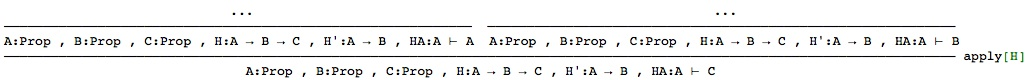
\includegraphics[width=\linewidth]{applyH.jpg}
  \caption{The portion of ProofWeb's tree visualization corresponding to the tactic ``\texttt{apply H}''.}
  \label{fig:applyH}
\end{figure}

\begin{figure}[h]
  \center
  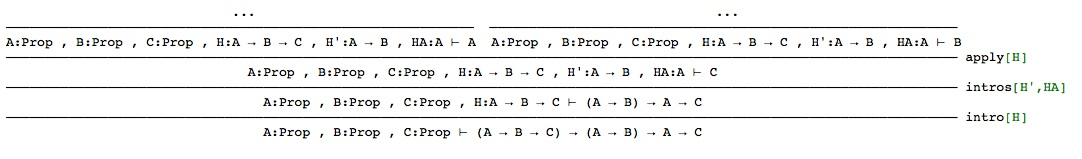
\includegraphics[width=\linewidth]{fullDisplayPartialTree.jpg}
  \caption{The partially completed tree from \autoref{fig:proofweb}, fully displayed.}
  \label{fig:fulldisplaypartialtree}
\end{figure}

The problems with current user interfaces that are discussed above are with respect to the scenario in which a novice user is inspecting an existing proof in order to determine the effects of various tactics under various conditions.  Many other scenarios with overlapping and related challenges also exist.  Such challenges include, but are not limited to,
\begin{itemize}
	\item locating particular items in a context (or in the larger environment)
	\item finding similar nodes in a proof tree
	\item deciding which tactic to apply
	\item keeping track of different proof attempts
	\item optimizing a proof or organizing a set of definitions, theorems and proofs for human understanding
	\item doing all these things efficiently. 
\end{itemize}



%%================================
\subsection{Coq User Interface Survey}
%%================================
Section \ref{currentUIproblems} described some usability problems that I, as a novice Coq user, noticed.  In this section, I describe an online survey (and its results) that Professor Juan Pablo Hourcade, Professor Aaron Stump, and I, in December 2011, invited subscribers to the Coq-Club mailing list to fill out.  This survey asked Coq users for their opinions and experiences regarding existing Coq user interfaces, and for their ideas regarding new interfaces.  Our motivation was both to validate our own ideas about new Coq user interfaces and to generate new ones.  We received 48 responses, including many detailed responses to the essay questions in the survey.

The survey consisted of 19 questions, of which 13 were multiple choice and the rest short answer or essay. The questions can be divided into three groups:  7 questions asking for background information on the respondent and how the respondent uses Coq, 9 questions asking for various ratings of the interface respondents use, and 3 open-ended questions directly related to the development of new user interfaces.  To these open-ended questions, we received many lengthy and thoughtful responses. \footnote{A more detailed survey report can be found at http://www.cs.uiowa.edu/~baberman/coquisuvey.html.}

The responses to the first group of questions showed a full range of (self-reported) Coq expertise levels, although a majority of responses indicated a high degree of expertise (on a scale going from 1=�novice� to 5=�expert�, 2 respondents rated themselves at level 1, 12 at level 2, 9 at level 3, 17 at level 4, and 8 at level 5).  9 respondents indicated they had been using Coq for less than 1 year, 27 for 1-5 years, 7 for 5-10 years, and 5 for more than 10 years.  Users of Proof General outnumbered users of CoqIDE 31 to 16.  24 respondents indicated using Coq for programming language or program verification research, 10 indicated using Coq for formalization of mathematics, and 8 indicated �teaching.� (There were 47 responses total to this free-response question.)

In the second group, to the question ``How satisfied are you with the interface you typically use?'', respondents gave a slightly positive average response (4.6 on a 1 to 7 point scale).  This was somewhat surprising to us at first, but it may have been an artifact of how the the question was asked.  For one thing, we did not present any sort of alternative interface, and current interfaces are, in fact, a significant improvement over the basic command prompt.  A second factor may be that many respondents have become accustomed to their current interface and may have viewed the question as asking how willing they would be to learn to use a new interface.  More than 25\% of respondents, however, did indicate some level of dissatisfaction.  Furthermore, answers to four questions revealed difficult tasks for users.  These questions asked users how difficult it is, using the interface they typically use, to 
\begin{itemize}
\item understand the relationships between subgoals, 
\item switch back and forth between potential proofs of a subgoal, 
\item compare similar subgoals, and 
\item tell what options for proving a subgoal are available. 
\end{itemize}
On a scale where 1=``Very Difficult'' and 7=``Very Easy'', the mean values for the answers to these questions were 2.74, 3.46, 2.35, and 2.57, respectively.   Responses to a fifth question, �How difficult is it for you to (mentally) parse Coq syntax?�, produced a mean value of 5.02 on the same scale, with only 4 responses indicating �Difficult� or �Somewhat difficult�.  Again, this may have been an artifact of the way the question was asked--how difficult, compared to what?

In the third group, we received almost 4,500 words (total) in response to the questions  
\begin{itemize}
\item ``What information would you like to have more readily available when working with Coq?'',
\item ``What do you think are the hardest parts of learning interactive theorem proving with Coq?'', and
\item ``What advice/requests/ideas do you have for creating better Coq user interfaces?''
\end{itemize}
Because of this volume, I categorized the responses to each question.

For the first question, the first category was ``library documentation.'' Respondents noted that Coq's ``\texttt{SearchAbout}'' command is a little hard to use, that they would like more simple examples of using Coq commands, that theorem names are not very readable, and that they would like integration of documentation, a la the Eclipse IDE's javadoc support.\footnote{For the reader not familiar with Integrated Development Environments, which are essentially text editors with features specialized to programming in various languages.  Eclipse\cite{Eclipse} is one of the more popular IDEs for Java programming.}  The second category was ``available tactics''/``relevant lemmas, relevant definitions'': respondents wanted the names of previously proved statements they could apply and, additionally, whether a tactic could be used to automatically prove either the the current goal or its negation.  The third category was information on terms, e.g. the type of a term, the value to which it reduces, or other implicit information (such information can already be made available by using commands like ``\texttt{Check}'' and ``\texttt{Print}'').  The fourth category was proof structure, including information on the relationships both between goals within a proof and between theorems and definitions.  Miscellaneous responses included similarities between terms, differences between terms and expected terms, and tactic debugging with custom breakpoints.

For the question ``What do you think are the hardest parts of learning interactive theorem proving with Coq?'', the first category of response was type theory-- that learning the type theory behind Coq is one of the hardest parts.  The second category had to do with lack of good tutorials.  The third category was that there are numerous poorly documented commands (again, the need for simple examples was mentioned).  Finally, the fourth category was proof readability, e.g. lack of support for mathematical notation and proof script organization.

For the question ``What advice/requests/ideas do you have for creating better Coq user interfaces?'', the first category was programming IDE features (e.g. auto-indentation, safe and correct renaming of identifiers, refactoring of tactics and groups of tactics, and background automation).  The second category was proof structure--representing proof structure by for instance grouping sibling goals, and allowing more flexibility to the order in which one works on goals.  The third category was syntax, which included having better ways to indicate where one wants to rewrite part of a term or where one wants to unfold a definition and automatic naming of hypotheses.  Some miscellaneous suggestions were to make more use of the mouse, avoid unnecessary re-execution of potentially long-running commands, and to have different editing and presentation tools.   

Even given the responses from self-described novice Coq users, the group of respondents is still heavily biased towards acceptance of arcane, complicated software.  The responses summarized above demonstrate that, even by this group, room for improvement is seen.

%%=======================================================================================
\section{Proposed and Completed Research}
%%=======================================================================================
%%================================
\subsection{Overview}
%%================================

In this section, I describe CoqEdit, three extensions to CoqEdit, and plans for evaluating two of these extensions with human participants.  As an interlude in the descriptions of the extensions, I include a presentation of the development and testing ``Keyboard-Card Menus'' as these are a component of one of the planned extensions.

%%================================
\subsection{CoqEdit}
%%================================

CoqEdit is a new user interface of Coq, that I, along with Harley Eades and under the supervision of Professors Juan Pablo Hourcade and Aaron Stump, have been developing. CoqEdit is a plugin to the \textit{jEdit}\cite{jEdit} text editor, a free and open source editor editor written in Java.\footnote{Another jEdit plugin, \textit{Isabelle/jEdit}, has been developed to provide support for the Isabelle\cite{Isabelle} interactive theorem prover and is bundled with Isabelle itself; see, for instance, \cite{wenzel2012asynchronous}.  Note that it has a rather different, and arguably more advanced, ``asynchronous'' style of interaction.  While this style of interaction may one day be available to Coq users, for now we are concentrating on other issues.}  For the most part, interaction with CoqEdit, at least in its unextended form, imitates the style seen with Proof General and CoqIde.  

\autoref{fig:coqedit} shows an initial version of the plugin.  This initial version is functional in that one can communicate with the \texttt{coqtop} command prompt by moving the highlighting forwards and backwards (using submenu items not seen in figure 6, or the items' shortcuts) to send messages to \texttt{coqtop}, which can then respond by changing the text printed in the two panels on the right.  It also allows allows \texttt{coqtop} to be interrupted when processing long-running commands, and includes the XML files telling jEdit how to do syntax highlighting for Coq's .v (``Vernacular'') files.  Note that these two panels actually sit within a jEdit ``dockable window'', which may be hidden (i.e. collapsed so that only its labeling tab is showing), undocked (i.e. made to float as a normal window), or docked in some other position (e.g. below the area containing text, instead of to its right).

\begin{figure}[h]
  \center
  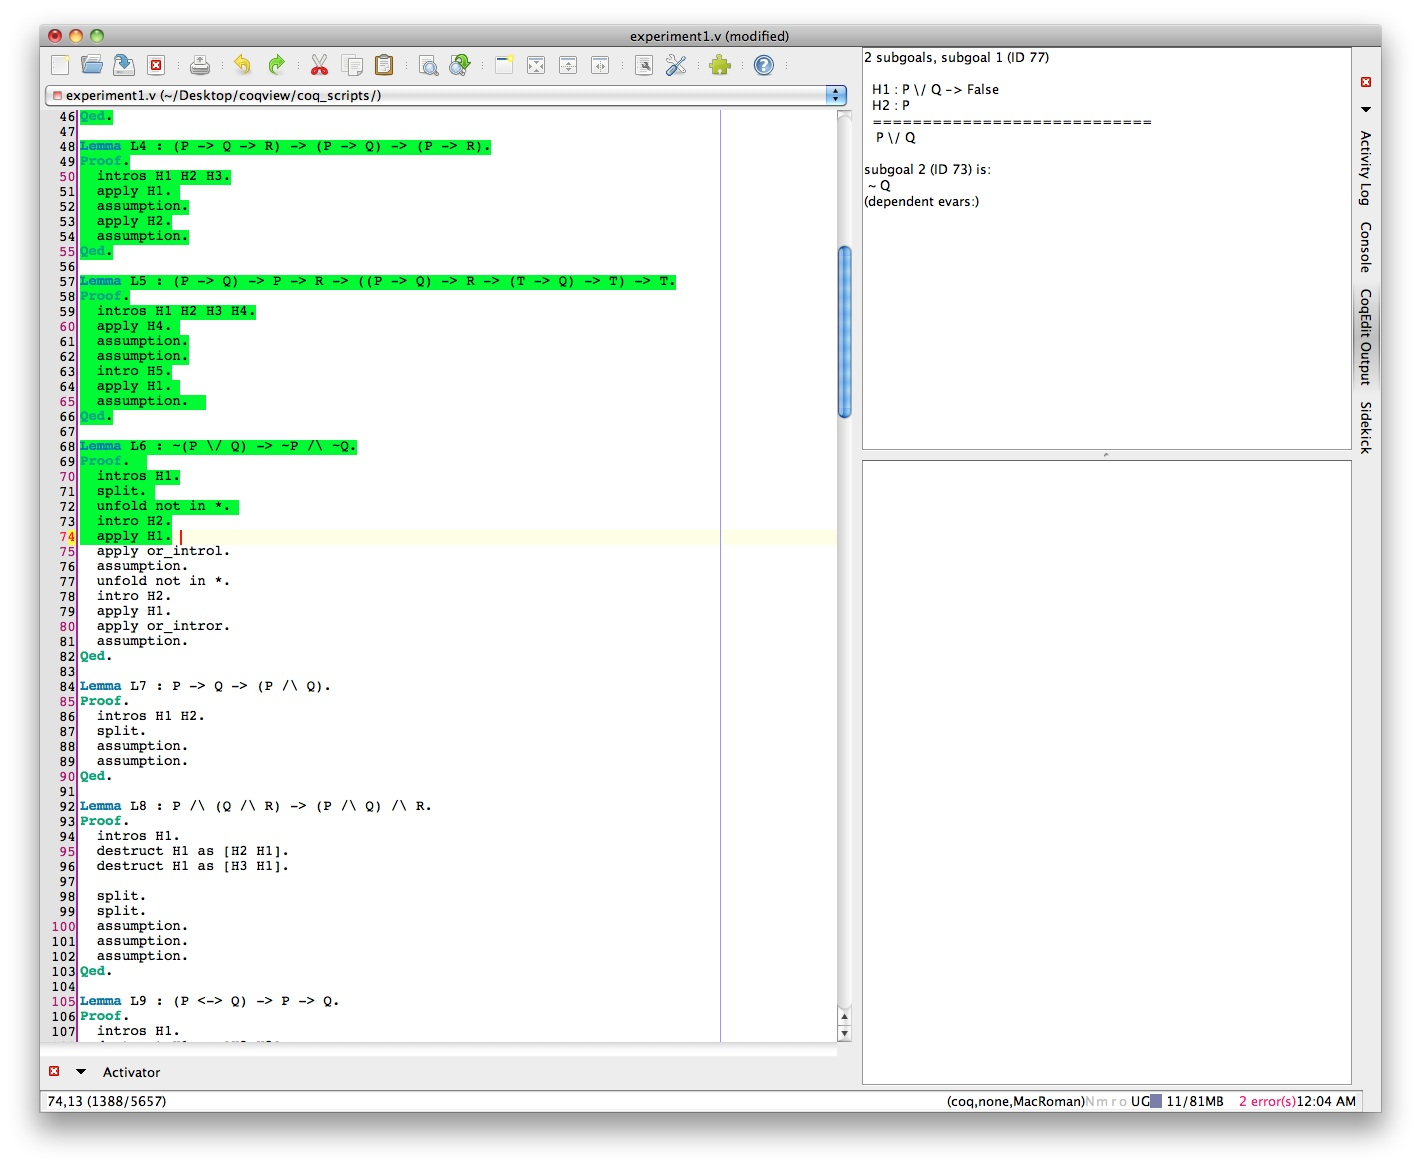
\includegraphics[width=1.1\linewidth]{coqedit.jpg}
  \caption{An initial version of CoqEdit.}
  \label{fig:coqedit}
\end{figure}

Although it does not contain some of the language-specific features of IDEs like Eclipse, jEdit does contain several noteworthy ones, besides its support for plugins.  These include syntax highlighting and auto-indentation for numerous languages, word completion, abbreviations, folding and many others (see the jEdit homepage\cite{jEdit}, and the features page to which it links).  The fact that jEdit runs on a Java Virtual Machine allows it to be used with Mac OS X, OS/2, Unix, VMS and Windows, and should also make extending CoqEdit support to multiple platforms relatively easy (I am currently developing it just under Mac OS X, but I expect it to immediately work just as well on Linux). Particularly important for the development of plugins is its BeanShell scripting language for writing macros, essentially an interpreted version of Java that makes experimentation with the jEdit API relatively easy, especially for Java programmers.  Plugins are, for the most part, actually collections of BeanShell scripts that generally invoke compiled Java code.

One of the features of jEdit's plugin system is that one can specify dependencies between plugins.  If plugin \textit{A} is specified as depending on plugin \textit{B}, then activating\footnote{``Loading'' a plugin does not necessarily ``activate'' it.}  \textit{A} in the plugin manager automatically activates \textit{B}.  This allows code from \textit{B} to be invoked from \textit{A}.  This makes it possible to write extensions to CoqEdit as jEdit plugins that allow features to be added incrementally and in various combinations.  In a nutshell, we can write plugins that plug into our CoqEdit plugin.

Currently, I am working on a major revision of the initial version shown in \autoref{fig:coqedit}.  Although this revision will include bug fixes and implement a few remaining unimplemented features, its main purpose is to improve the software architecture in order to make future CoqEdit extensions easier.  \textit{This foundation for future user interface research will be one of the major contributions involved in this dissertation.}  It will make taking advantage of the extensive Java libraries, particularly those for 2D graphics, and of the Java development community's expertise, much more straightforward.

This new, still quite basic, user interface will however improve upon Proof General and CoqIde in a couple of different ways.  First, it will cache the output of sentence evaluation and allow a window into this cache using movable dark green highlighting of a sentence within the evaluated region (Proof General caches this output, but requires users to hover over the text with the mouse to make a tooltip with it appear).  Second, it will allow both multiple instances of \texttt{coqtop} to run simultaneously \textit{and} multiple text areas to show multiple areas within a buffer that is being evaluated. 


%%================================
\subsection{CoqEdit Extensions}
%%================================

%%============
\subsubsection{``Proof Previews''}
%%============

Our first experimental extension, ``Proof Previews'', is shown in \autoref{fig:proofpreviews}.  When the user presses CTRL-SPACEBAR while the system is in proof mode, a popup window containing a list of possible tactic/argument combinations (i.e. ones that do not immediately produce errors or take especially long to run) appears just below the end of the evaluated section.  The user can use the up and down arrow keys change the selected item in the list and the ENTER (or ``return'') key to insert the selected item into the script.  In addition, the output that would result from evaluating the selected item is displayed in the bottom output panel.  The general goal of this plugin is to allow users, novice users in particular, to quickly explore their available options.


\begin{figure}[h]
  \centering
  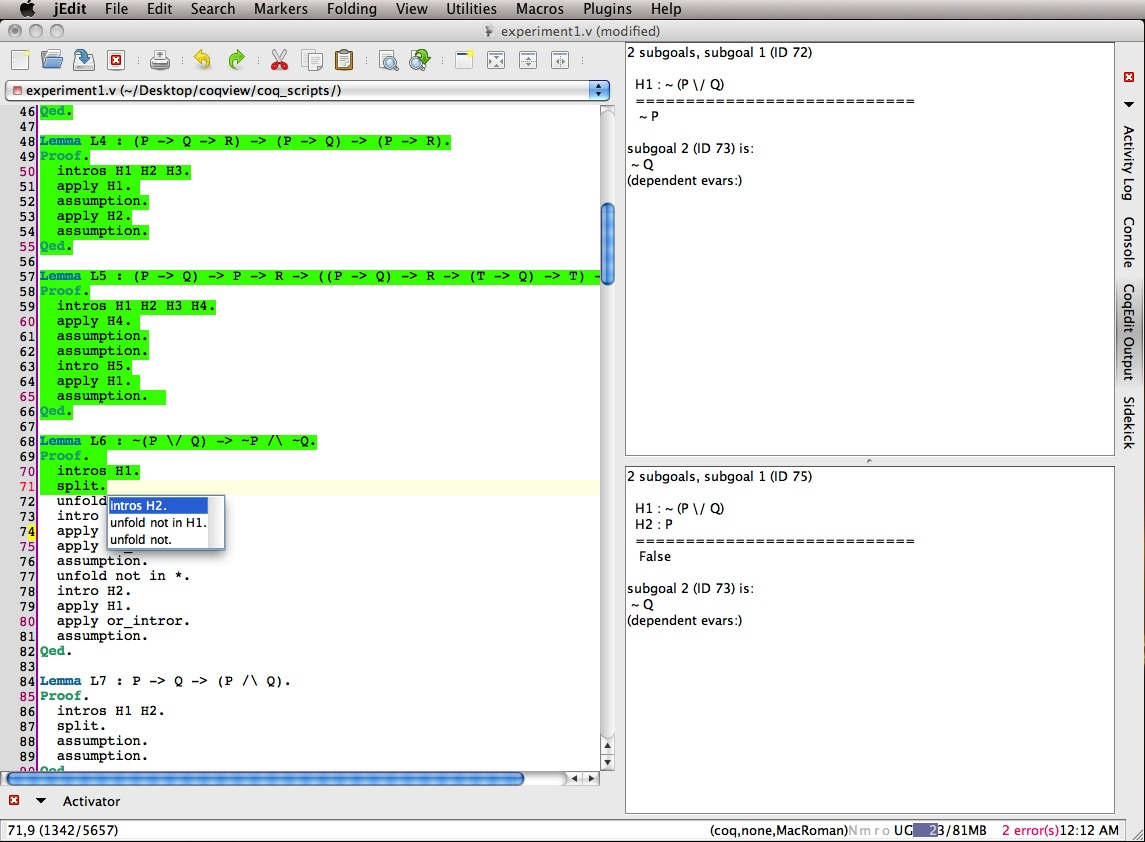
\includegraphics[width=1.1\linewidth]{proofpreviews.jpg}
  \caption{CoqEdit with the Proof Previews extension.  The result of the highlighted tactic is displayed in the bottom output panel.}
  \label{fig:proofpreviews}
\end{figure}

The tactic list generation capabilities for this plugin are quite limited at the moment:  only tactics used in propositional logic exercises and examples may appear in the list.  While this may still be useful for educational purposes, our implementation is mainly to be used for usability testing and to demonstrate the utility of the general idea.  A more fully developed version of this plugin would be possible, but would likely require some complicated indexing of Coq's standard library.  

%%============
\subsubsection{``Proof Transitions''}
%%============

Our second experimental extension, ``Proof Transitions'', evolved from two separate ideas.  The first is proof tree visualization.  Originally, we proposed visualizing Coq's proof trees as in \autoref{fig:prooftreebuild}, where 
\begin{itemize}
\item the red half circles represent goals, 
\item the blue half circles, placed on top of the red half circles to form complete circles, represent tactics successfully used with the goals corresponding to these red half circles, 
\item child goals are arranged \textit{above} parent nodes (as in \autoref{fig:fulldisplaypartialtree}),
\item thin red lines connect parent nodes to unproved child branches, 
\item thick black lines connect parent nodes to proved child nodes, and
\item the yellow arrow represents the current node.
\end{itemize}
(\autoref{fig:prooftreebuild} visualizes the example from section \ref{examplesection}).

In addition to helping users in seeing which child goals are associated with which parent goals and tactics, and potentially in traversing/adding the trees' nodes in arbitrary orderings, this sort of visualization could be enhanced further to provide valuable information.  For instance, \autoref{fig:similarnodes} shows nodes being highlighted based on similarities in the tactics \footnote{...which might be particularly helpful in avoiding loops proofs}.  The information associated with these nodes could be compared side-by-side using an additional output window whose location within the proof tree could be represented by an additional arrow, as in \autoref{fig:nodecomparison}.  

\begin{figure}[H]
  \center
  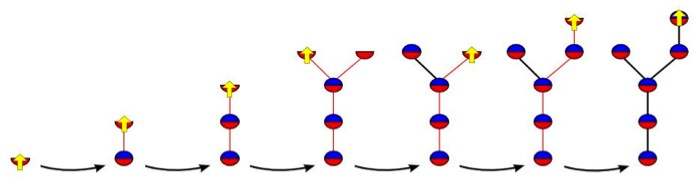
\includegraphics[width=1.1\linewidth]{prooftreebuild.jpg}
  \caption{A series of partial proof tree visualizations of the example of section \ref{examplesection}, in an earlier style.  }
  \label{fig:prooftreebuild}
\end{figure}

\begin{figure}[H]
  \center
  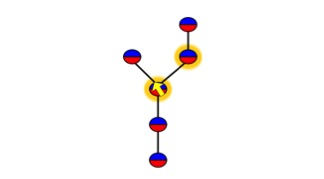
\includegraphics[width=0.7\linewidth]{similarnodes.jpg}
  \caption{Similar nodes being highlighted while the node under the yellow arrow is inspected.}
  \label{fig:similarnodes}
\end{figure}

\begin{figure}[H]
  \center
  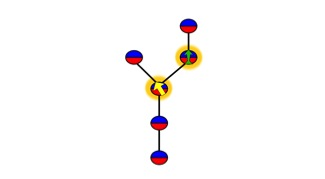
\includegraphics[width=0.7\linewidth]{nodecomparison.jpg}
  \caption{The proof tree visualization of \autoref{fig:similarnodes}, with an additional arrow to represent the location of another output window within the proof tree.}
  \label{fig:nodecomparison}
\end{figure}

Proof tree visualizations could also be enhanced to support management of different versions of proof tree branches, as in \autoref{fig:versionmanagement}, and to support proof presentation, as in \autoref{fig:} which shows how a branch deemed uninteresting might be removed from the visualization.  These examples suggest the existence of a wide range of possible user interface improvements that may not even have been thought of yet, and that are part of the rationale for making CoqEdit more easily extendable.

\begin{figure}[H]
  \center
  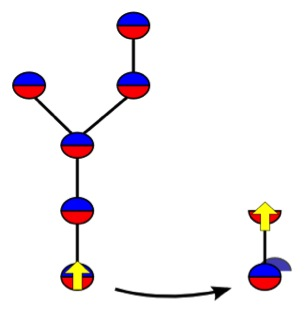
\includegraphics[width=0.35\linewidth]{versionmanagement.jpg}
  \caption{A user might decide to try an alternate proof of a branch (or the entirety) of the tree, or the entire tree.  A saved copy of the original branch might be represented by a ``shadowing'' blue half-circle, as seen on the right-hand side of this figure.}
  \label{fig:versionmanagement}
\end{figure}

\begin{figure}[H]
  \center
  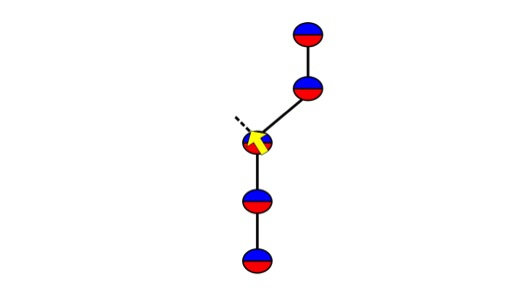
\includegraphics[width=0.7\linewidth]{presentationmanagement.jpg}
  \caption{The visualization of \autoref{fig:similarnodes}, with a branch hidden.  This sort of hiding might be useful in making the structure of the remaining visible branches more clear.}
  \label{fig:versionmanagement}
\end{figure}


The second idea from which the Proof Transitions extension evolved was ``Inference Rule Highlighting''.   The idea here is to use highlighting the to show the pattern, or inference rule, being instantiated by a tactic application on a goal.  In \autoref{fig:inferenceruleinstance}, we see an instance of the general rule seen in \autoref{fig:inferencerule}.  The blue box contains a tactics while the red box below contains the old goal and the red box above contains the new goal (in general, one might see several red boxes above).  The goal is for users to be able to clearly see the effects of tactics on particular goals, i.e. which bits of text get moved where, and for novice users to gain an understanding of how the tactic works more generally.


\begin{figure}[H]
  \center
  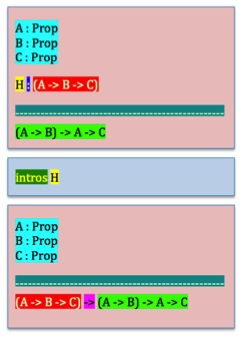
\includegraphics[width=.45\linewidth]{inferenceruleinstance.jpg}
  \caption{Inference Rule Highlighting example:  child, parent, and tactic, with highlighting showing where the tactic has moved and added text.}
  \label{fig:inferenceruleinstance}
\end{figure}


\begin{figure}[H]
  \center
  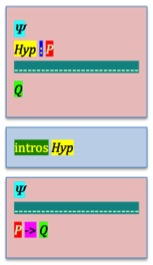
\includegraphics[width=.25\linewidth]{inferencerule.jpg}
  \caption{The general inference rule on which \autoref{fig:inferenceruleinstance} is based.}
  \label{fig:inferencerule}
\end{figure}


This particular way debugging tactics may work for many of the basic tactics, but it does not scale very well to more complicated tactics, since, for one thing, one eventually runs out of easily-distinguishable colors, and many tactics do not correspond to simple general rules of the like that seen in \autoref{fig:inferencerule} (e.g. the \texttt{auto} tactic that tries to automatically prove a goal).  Proof Transitions will provide an alternative which, in an initial form, can be seen demonstrated in \autoref{fig:pt1}, \autoref{fig:pt2}, \autoref{fig:pt3}, and \autoref{fig:pt4}.  \autoref{fig:pt1} shows the initial goal.  \autoref{fig:pt2} shows how immediately after the tactic \texttt{intros H1 H2} has been processed by the system, a blue box, containing the tactic, is placed immediately on top of the old goal and the new goal, in another red box, is placed further up with a line connecting its red box and the blue box.  As an option, as seen in \autoref{fig:pt3}, highlighting and underlining can be added to the boxes' text according to the following rules:  
\begin{itemize}
\item red highlighting in the bottom red box to show text that is deleted altogether, 
\item green highlighting in the top red box to show text that is entirely new, 
\item yellow highlighting in any box to show text that is moved (or copied, in the case of identifiers given as the tactic arguments),
\item red underlining in the bottom red box to show text that is either moved or deleted altogether, and 
\item green underlining in the top red box to show text that is new (either entirely new or moved/copied into the box)
\end{itemize}
In addition, the user can have lines, or arrows, drawn to connect the moved/copied portions of text, as seen in \autoref{fig:pt4}.  Note that within the program the lines are drawn one-by-one in an animation, which makes it easier to see what is connected to what than what might appear to be the case just  looking at \autoref{fig:pt4}

\begin{figure}[H]
  \center
  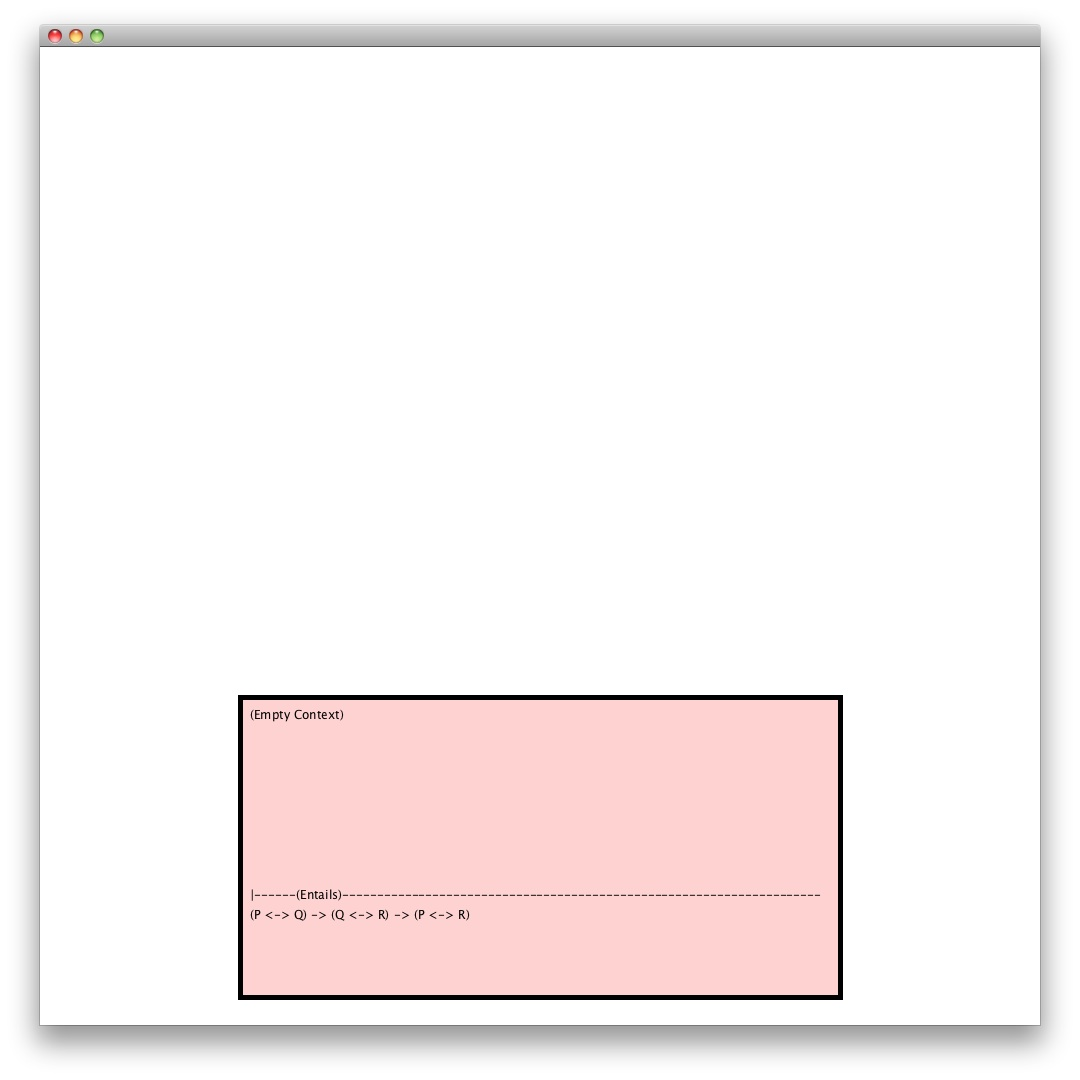
\includegraphics[width=\linewidth]{pt1.jpg}
  \caption{Proof transitions: a goal, pre-transition}
  \label{fig:pt1}
\end{figure}

\begin{figure}[H]
  \center
  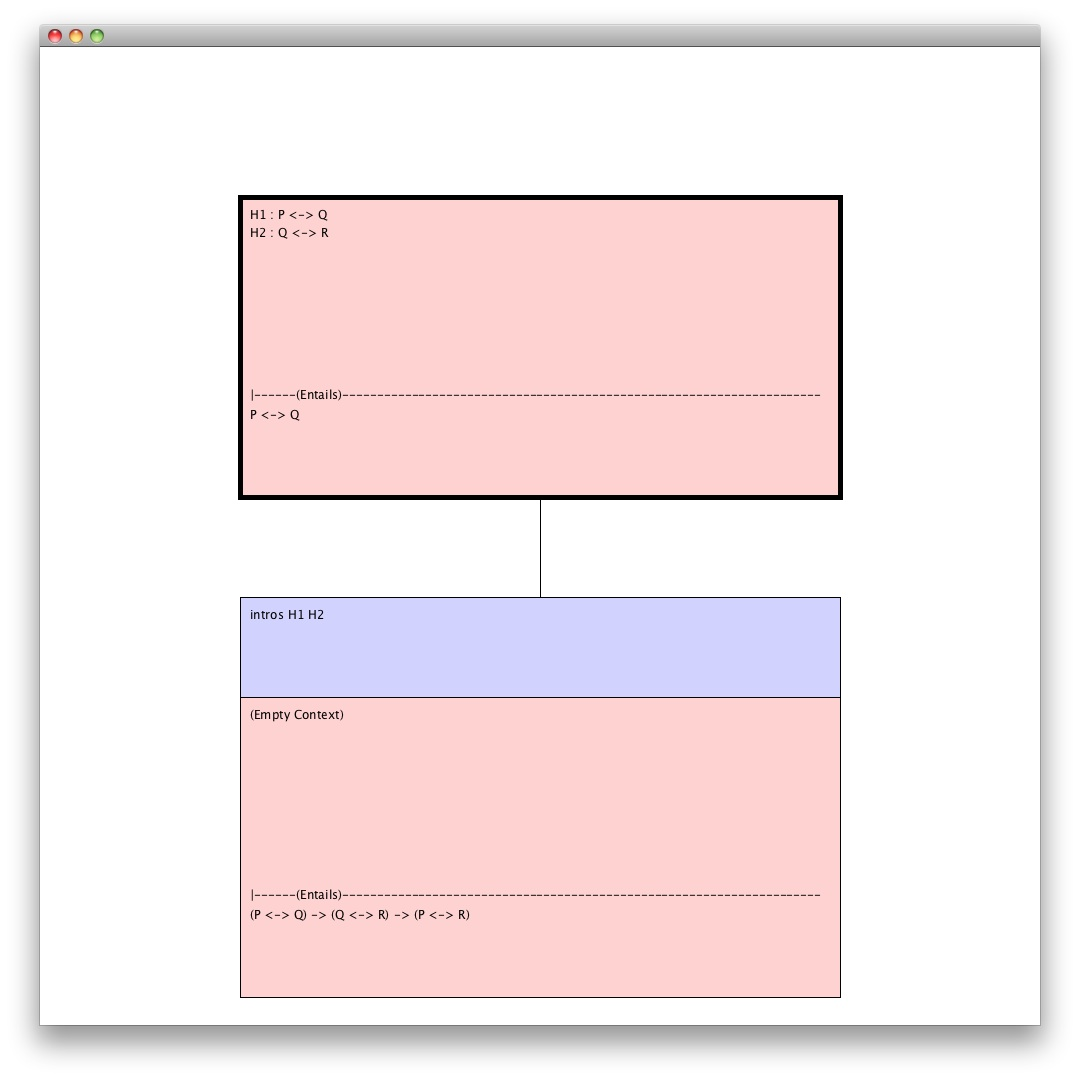
\includegraphics[width=\linewidth]{pt2.jpg}
  \caption{After a tactic has been applied to the goal in \autoref{fig:pt1}, stage 1.}
  \label{fig:pt2}
\end{figure}

\begin{figure}[H]
  \center
  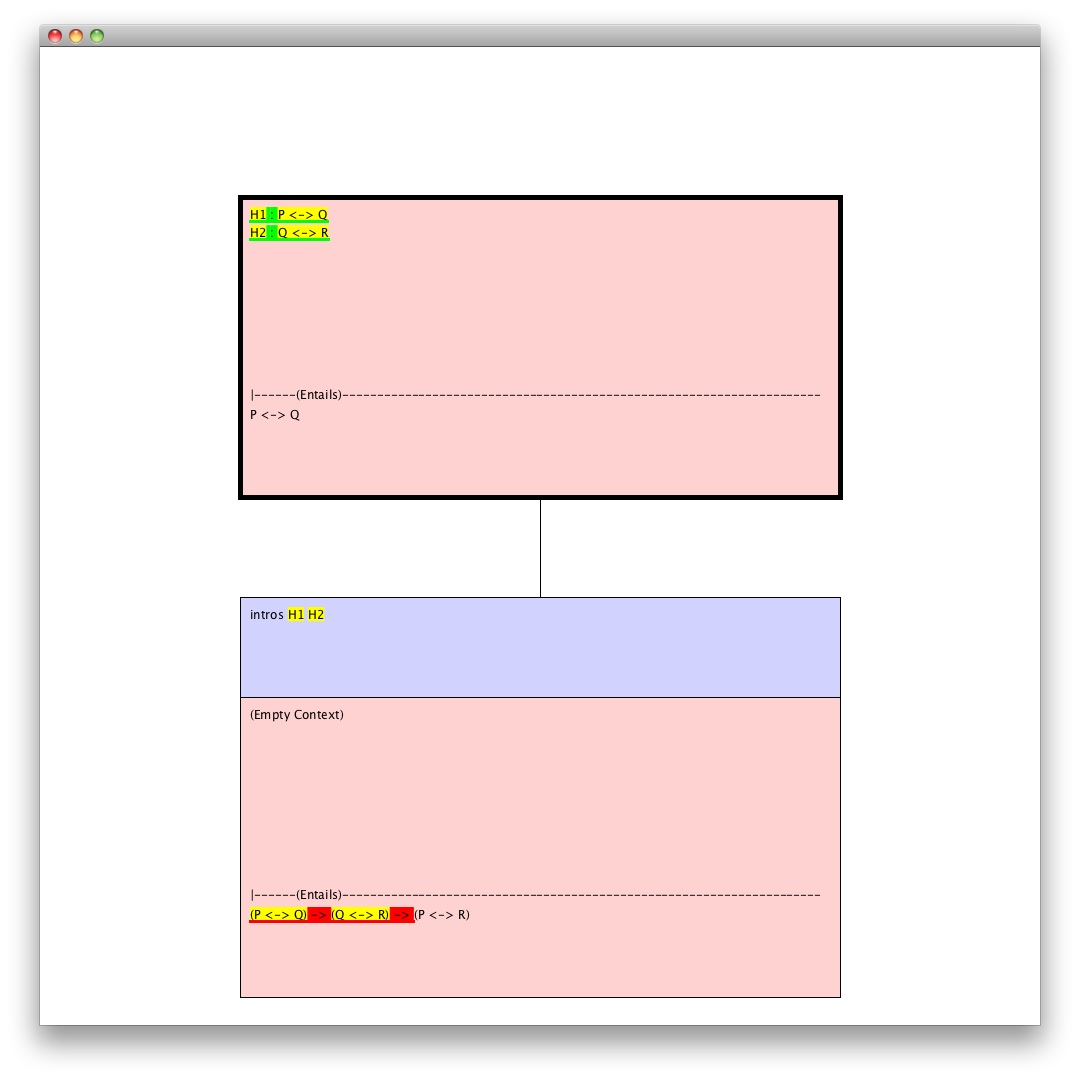
\includegraphics[width=\linewidth]{pt3.jpg}
  \caption{After a tactic has been applied to the goal in \autoref{fig:pt1}, stage 2.}
  \label{fig:pt3}
\end{figure}

\begin{figure}[H]
  \center
  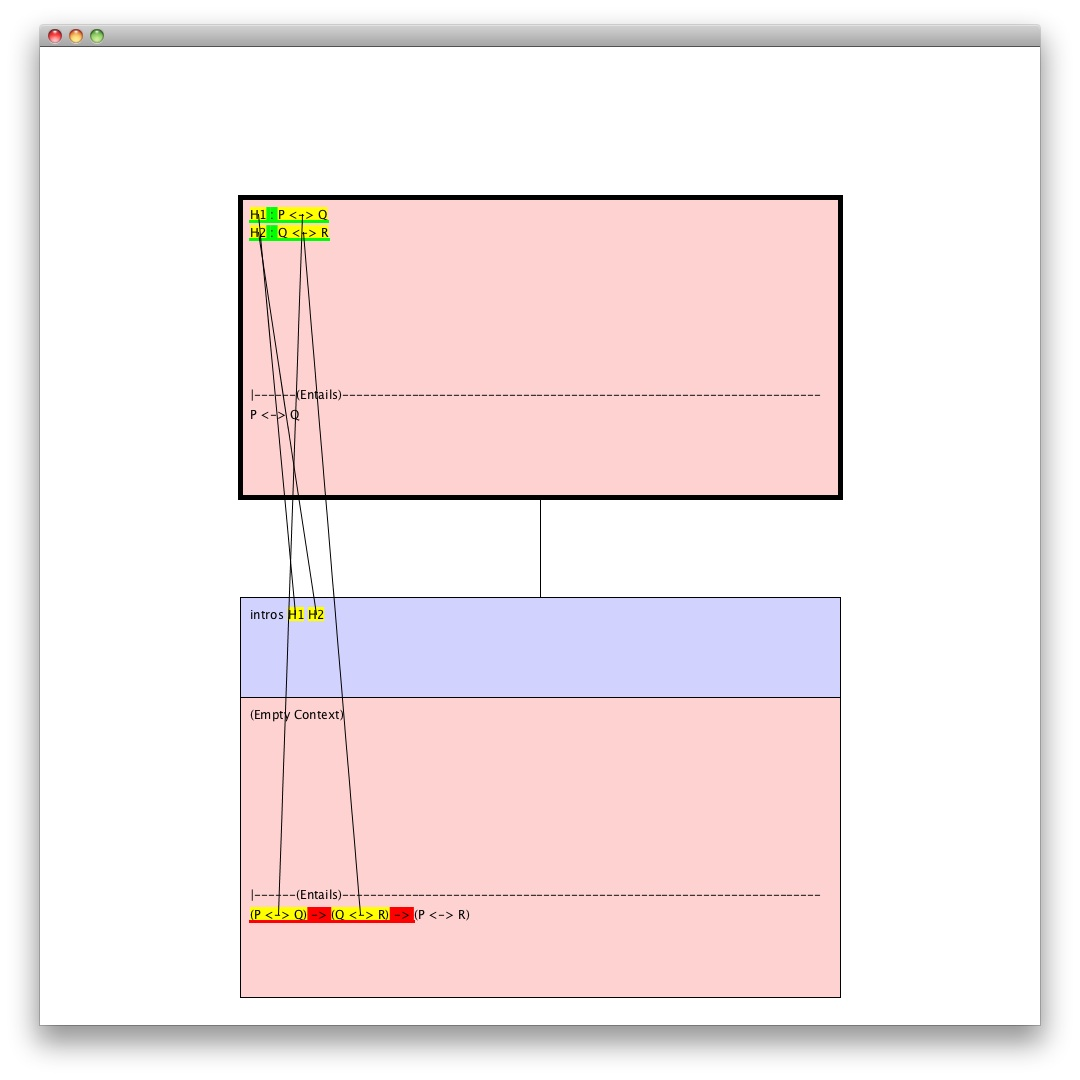
\includegraphics[width=\linewidth]{pt4.jpg}
  \caption{After a tactic has been applied to the goal in \autoref{fig:pt1}, stage 3.  Note that the lines would be added one at a time.}
  \label{fig:pt4}
\end{figure}


\begin{figure}[H]
  \center
  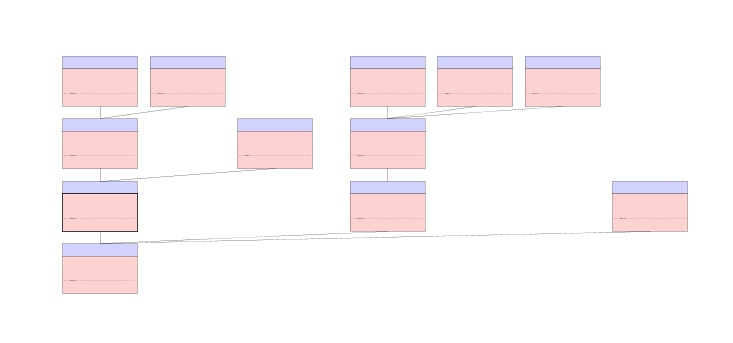
\includegraphics[width=\linewidth]{ptZoomOut.jpg}
  \caption{CoqEdit with the Proof Previews extension.  The result of the highlighted tactic is displayed in the bottom right panel.}
  \label{fig:ptZoomOut}
\end{figure}

\begin{figure}[H]
  \center
  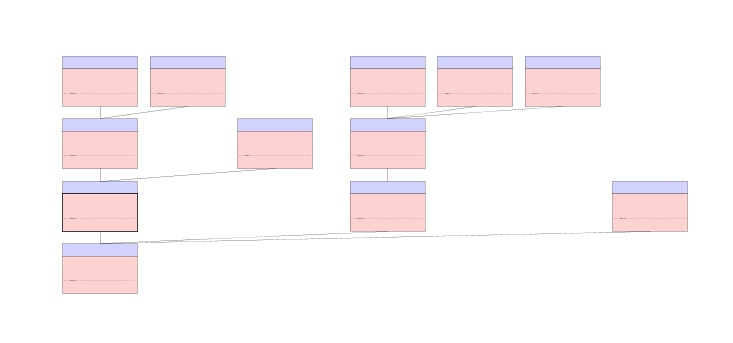
\includegraphics[width=\linewidth]{ptZoomOut.jpg}
  \caption{CoqEdit with the Proof Previews extension.  The result of the highlighted tactic is displayed in the bottom right panel.}
  \label{fig:ptZoomOut}
\end{figure}

%%================================
\subsection{Interlude: Keyboard-Card Menus}
%%================================

In this section, I describe work on ``Keyboard-Card Menus'', which I hope to incorporate into a third extension to CoqEdit.

%%================================
\subsection{CoqEdit Extensions, Continued}
%%================================

%%============
\subsubsection{``Propositional Logic Syntax Shortcuts''}
%%============

\begin{figure}
  \center
  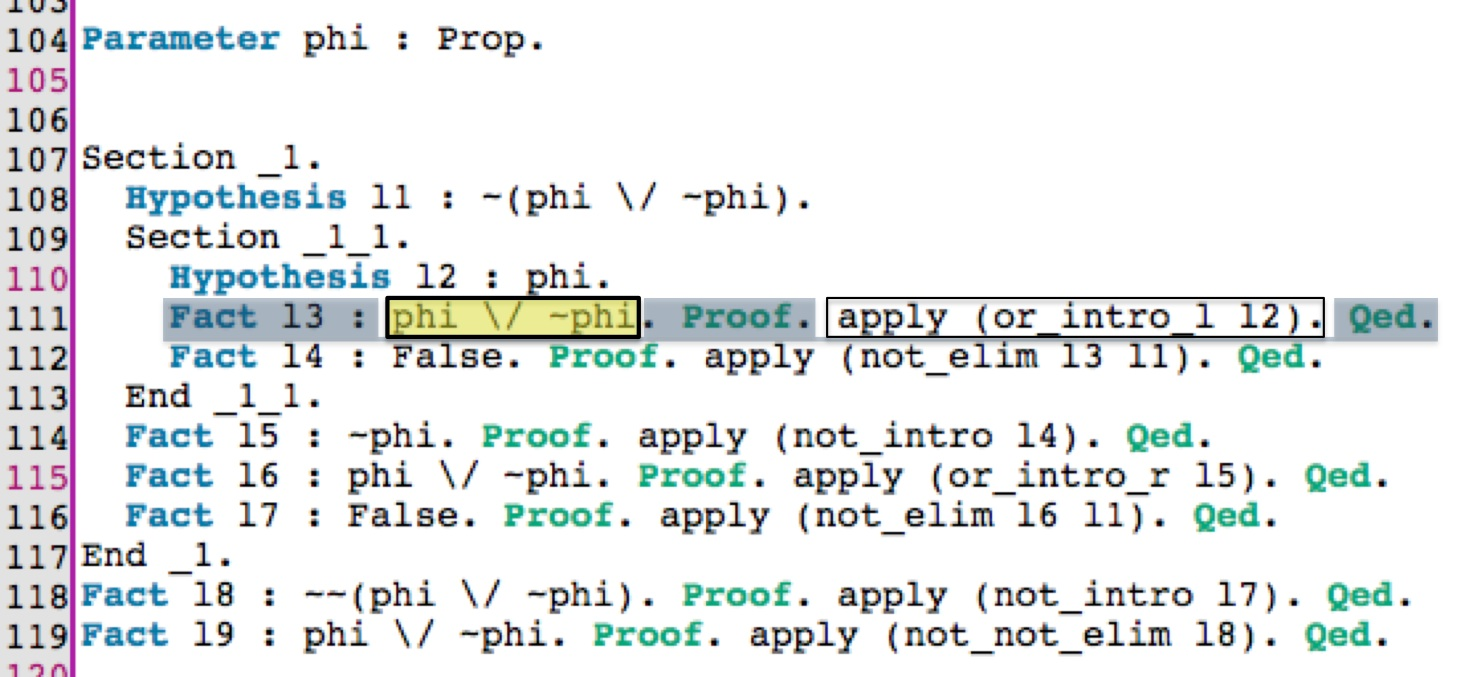
\includegraphics[width=\linewidth]{PLSS_1.jpg}
  \caption{Syntax Tree Highlighting for Propositional Logic Syntax Shortcuts}
  \label{fig:plss1}
\end{figure}

\begin{figure}
  \center
  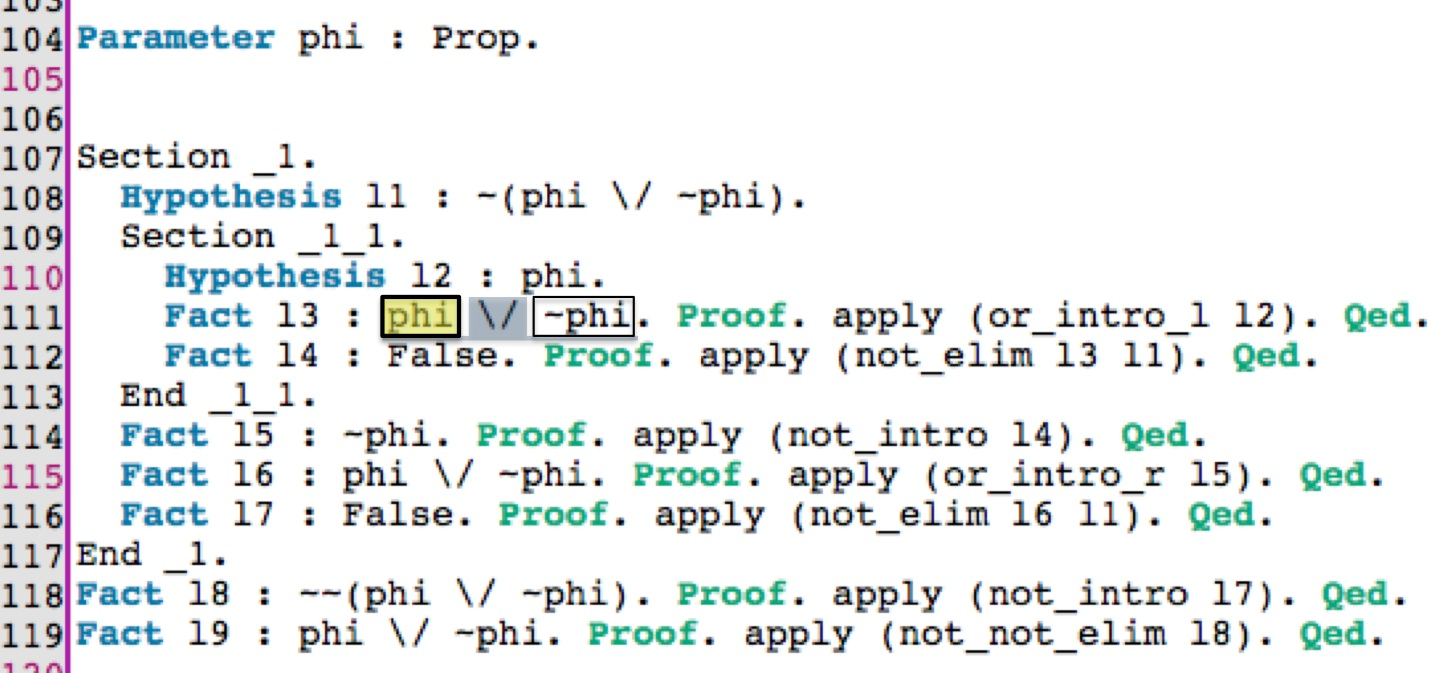
\includegraphics[width=\linewidth]{PLSS_2.jpg}
  \caption{Syntax Tree Highlighting for Propositional Logic Syntax Shortcuts, with highlighting moved from \autoref{fig:plss1}}
  \label{fig:plss2}
\end{figure}



%%================================
\subsection{Extension Testing}
%%================================

%%=======================================================================================
\section{Timeline for Research}
%%=======================================================================================



%%=======================================================================================
\section{Related Work}
%%=======================================================================================




%=======================================================================================
\section{Conclusion}
%=======================================================================================

I hope to have made several points in this proposal.  First, that this is important work, both because the Coq interactive theorem prover is an important tool that could benefit significantly from improved user interfaces and because many of the ideas generalize to other forms of coding.  Second, that as an intellectual challenge this work is non-trivial, not only because of the normal programming problems that must be overcome but because designing good user interfaces for complicated systems, which includes the identification of tractable problems and the testing of potential solutions, is non-trivial.  Finally, that, despite this non-trivial nature, the work can be accomplished.


%===================================================================================================
\bibliographystyle{plain}
\bibliography{refs}

\end{document}  